\documentclass{article}
\usepackage[utf8]{inputenc}
\usepackage[russian]{babel}
\usepackage{graphicx}
\usepackage{caption}
\graphicspath{{pictures/}}
\DeclareGraphicsExtensions{.pdf,.png,.jpg}
\begin{document}
\begin{center}
\hfill \break

\LARGE{Математический анализ}\\
\hfill \break
\normalsize{Модуль 3\\
\hfill \break
2021 год\\
\hfill \break
«Интеграл функции одной переменной»}\\
\hfill \break
\hfill \break
\hfill \break
\hfill \break
\end{center}

\begin{flushright} Иванов Сергей, Иванов Алексей, Титов Даниил \end{flushright}
\begin{flushright} M3104 \end{flushright}
\hfill \break
\hfill \break
\hfill \break
\hfill \break
\hfill \break
\hfill \break
\hfill \break
\hfill \break
\hfill \break
\hfill \break
\hfill \break
\hfill \break
\hfill \break
\hfill \break
\hfill \break
\hfill \break
\hfill \break
\hfill \break
\hfill \break
\hfill \break
\hfill \break
\hfill \break
\hfill \break
\begin{center} Май 2021 \end{center}
\begin{center} ИТМО \end{center}
\thispagestyle{empty} % выключаем отображение номера для этой страницы
\newpage
\tableofcontents{}
\newpage
\section{Интегральная сумма}
\normalsize
\subsection{Исследуйте интегральную сумму функции $f(x)$, заданной на отрезке $[a, b]$}
\\
$ f(x) = \sin{x} $\\
$ [a, b] = [0; 3\pi/2] $\\

Что мы сделали:\\
- Изобразили график функции\\
- Изобразили криволинейную трапецию, ограниченную графиком функции, вертикальными прямыми, проходящими через концы отрезка, и осью O$x$\\
- Разбили отрезок на $n$ элементарных отрезков, точками отметьте их концы на рисунке\\
- Выбрали по точке внутри каждого элементарного отрезка, отметили их на рисунке\\
- Вычислили значения функции в выбранных точках, отметили их на рисунке\\
- Изобразили ступенчатую фигуру на основе выбранного разбиения и точек внутри элементарных отрезков\\

\begin{figure}[h!]
\center{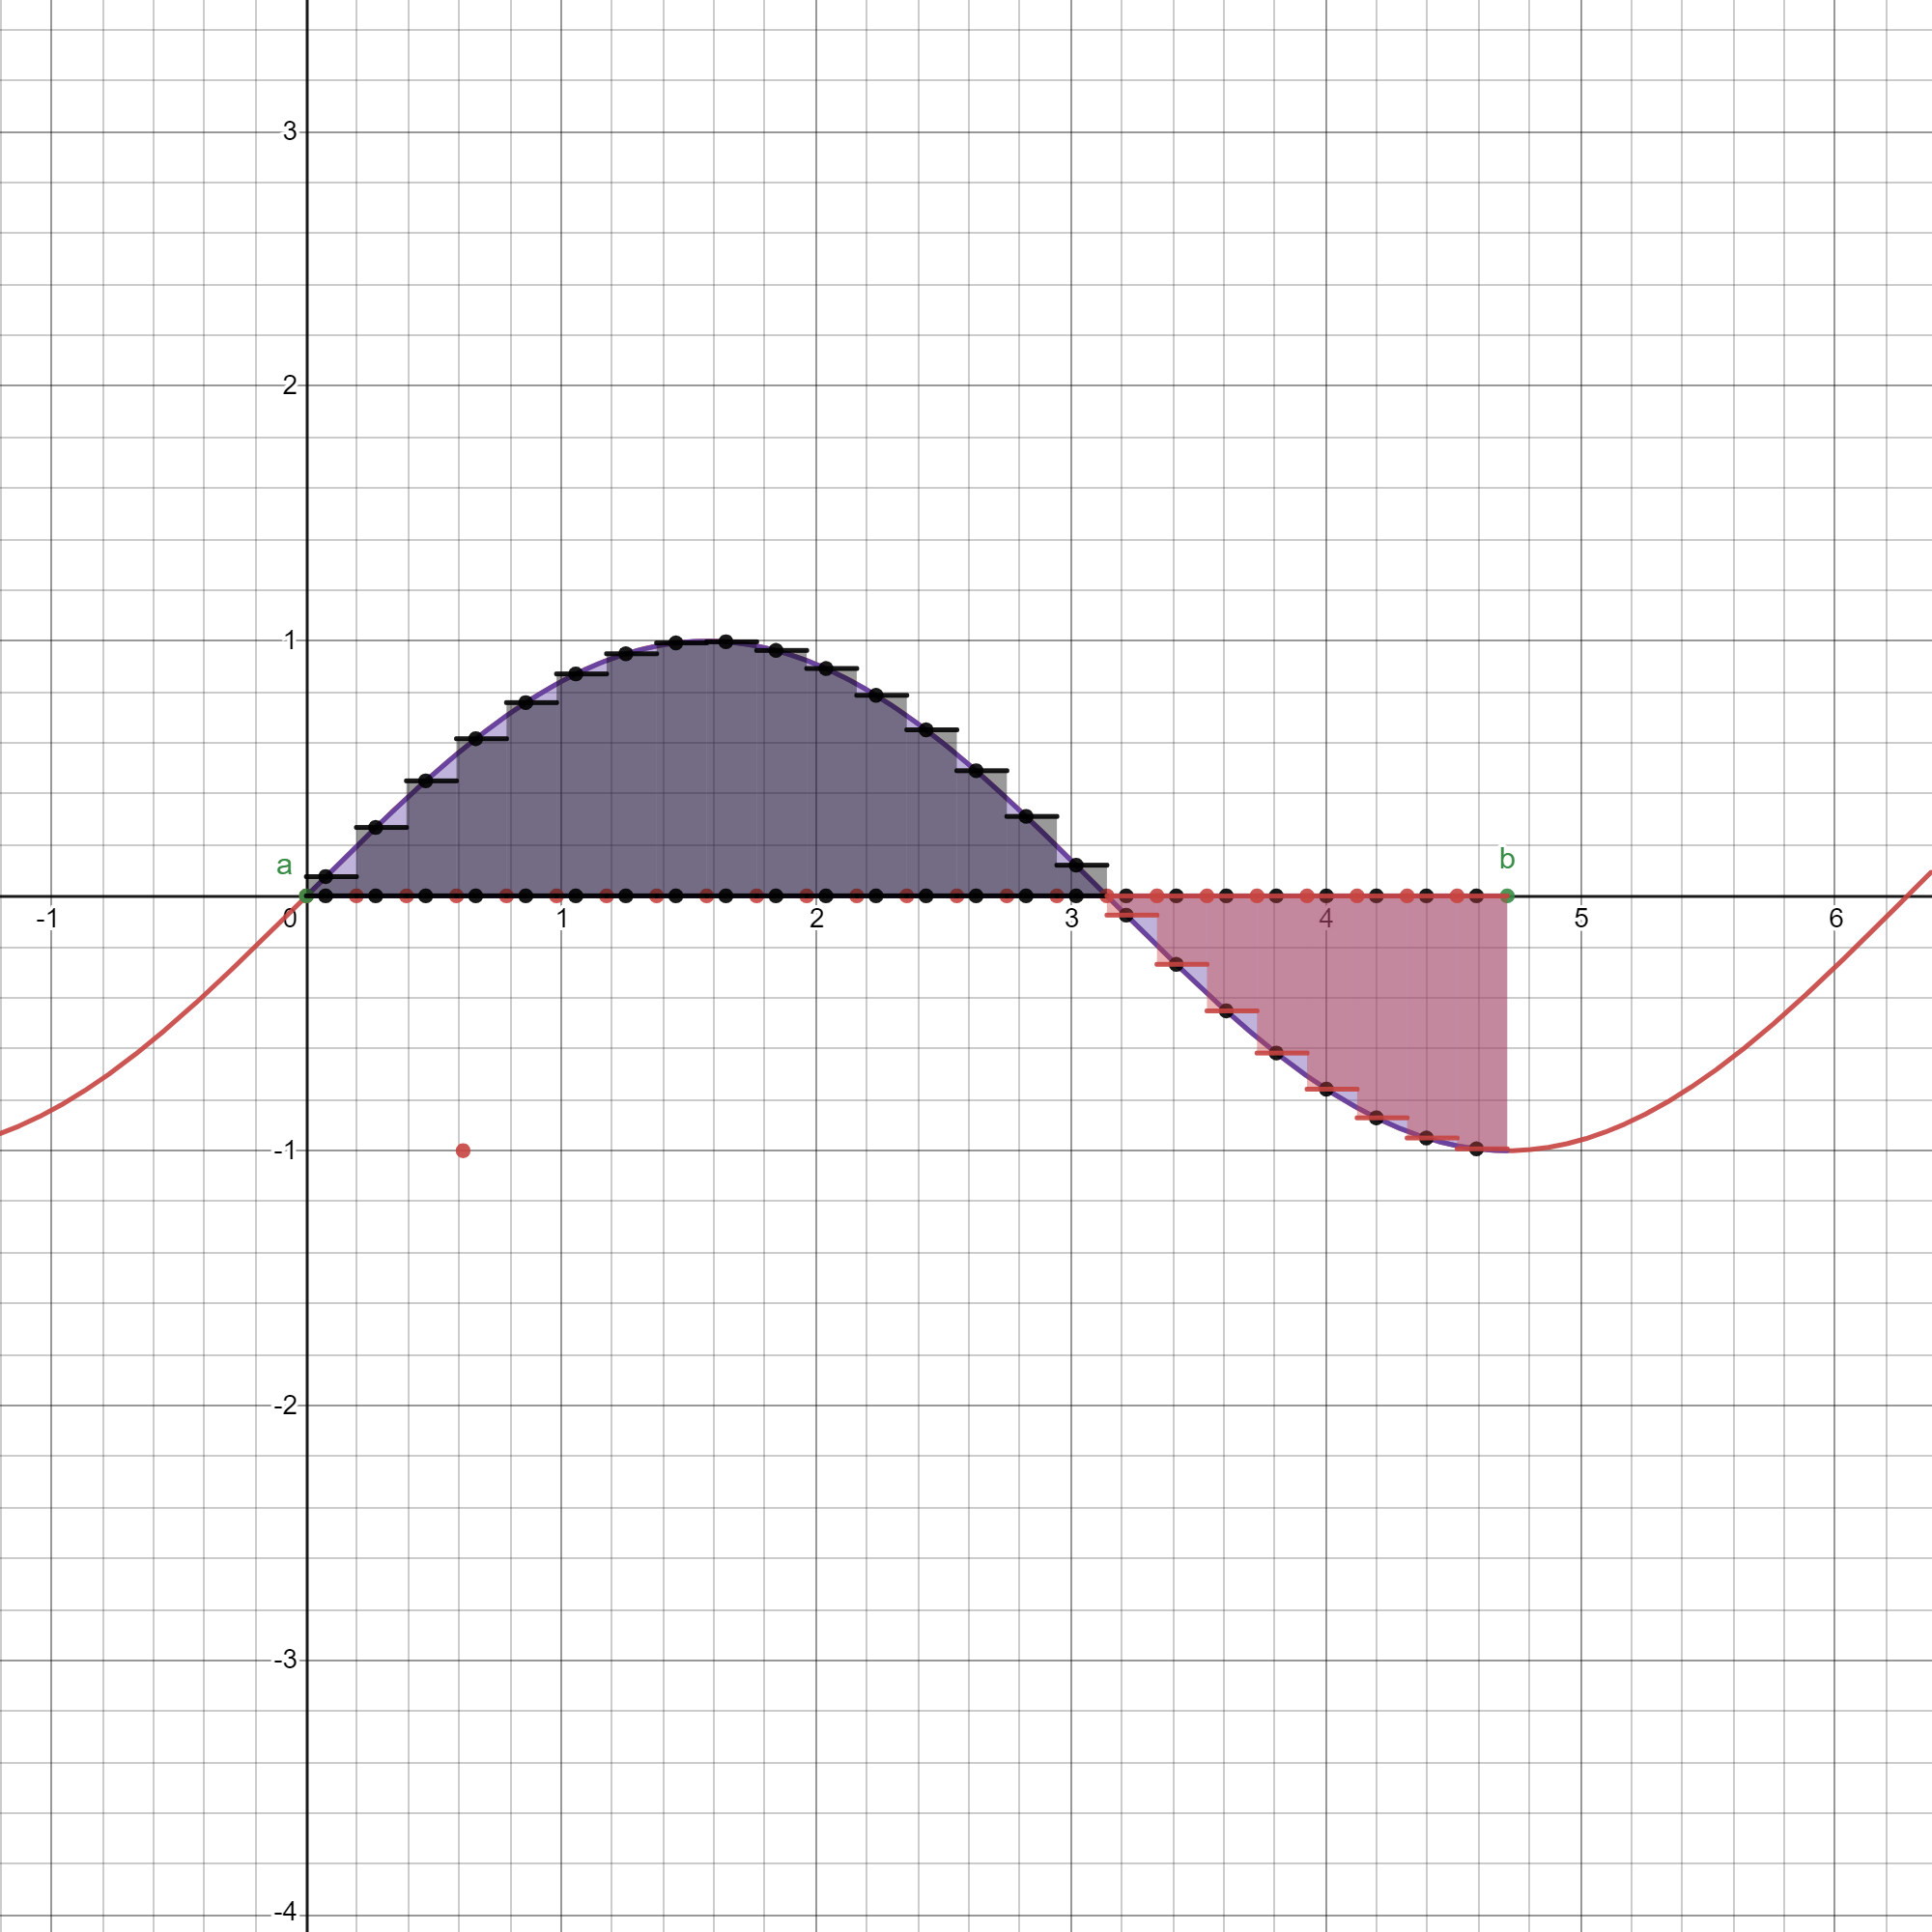
\includegraphics[scale=0.1]{1}}
\caption*{\url{https://clck.ru/UjTMB}}
\end{figure}
\newpage
\Large
\section{Несобственный интеграл}
\normalsize
\subsection{Исследуйте несобственный интеграл на сходимость при всех значениях параметра $ \alpha $}

\large $ \int\limits^{+\infty}_{1} \frac{\ln{x}}{x^{\alpha}}dx $\\
\normalsize

План:\\
1. Определите особую точку несобственного интеграла. Есть ли другие особые точки? К какому типу относится данный несобственный интеграл? Является ли подынтегральная функция неотрицательной на промежутке интегрирования?\\
2. Постройте графики подынтегральной функции при нескольких значениях параметра\\
3. Есть ли значение параметра, при котором легко находится первообразная? Если есть, то найдите её и сделайте вывод о сходимости интеграла\\
4. Сформулируйте признаки сравнения для определения сходимости несобственных интегралов\\
5. Оцените сверху и снизу трансцендентную функцию (логарифм или арктангенс) для сравнения исходного интеграла с интегралом вида. Установите, при каких значениях параметра это сравнение позволяет сделать вывод о сходимости интеграла\\
6. Вспомните, как ведёт себя интеграл при значении параметра, при котором легко находится первообразная. Используйте этот интеграл как эталон для сравнения с интегралом при другом параметре $ \alpha $ \\
7. Запишите ответ\\
\\\\
1. Особая точка: $ x = 1 $, так как значение функции в ней всегда равно $ 0 $\\
Подынтегральная функция не является неотрицательной на промежутке интегрирования\\\\
2. \\
\begin{figure}[h!]
\center{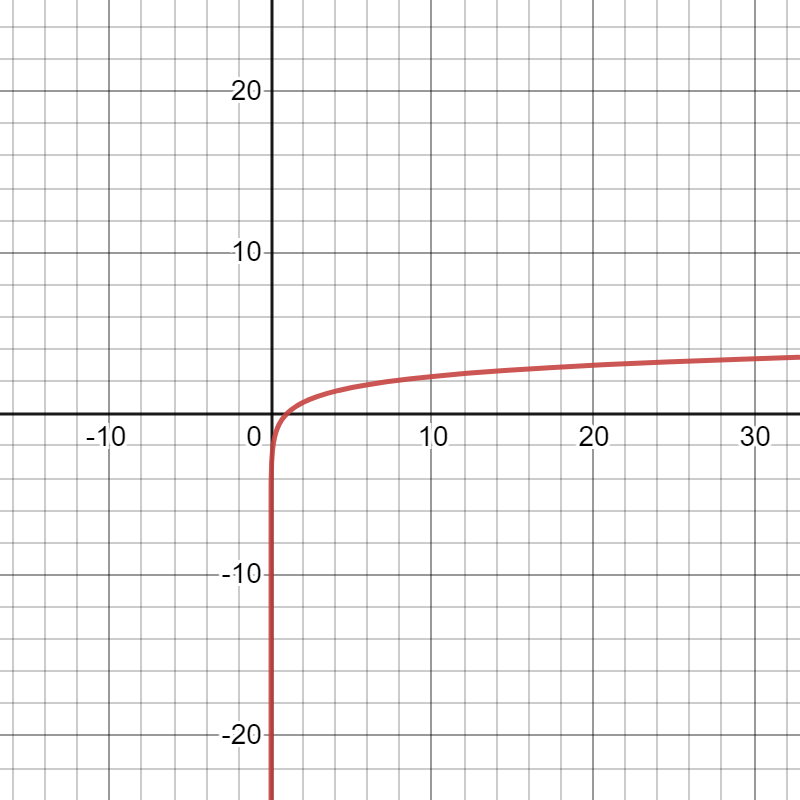
\includegraphics[scale=0.15]{20}}
\caption*{$ \alpha = 0 $}
\end{figure}\\
\begin{figure}[h!]
\center{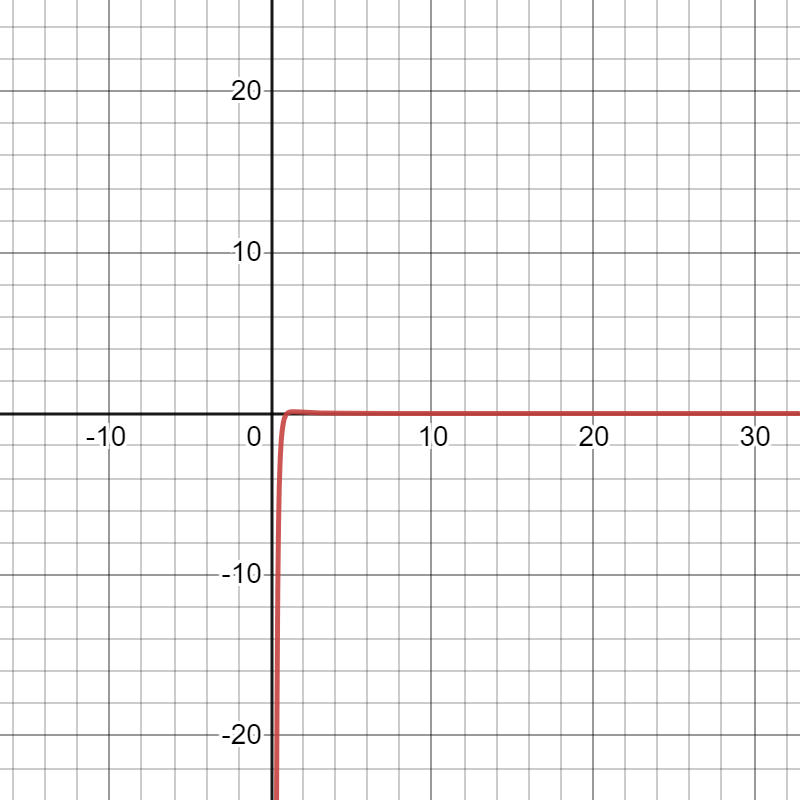
\includegraphics[scale=0.15]{23}}
\caption*{$ \alpha = 3 $}
\end{figure}
\begin{figure}[h!]
\center{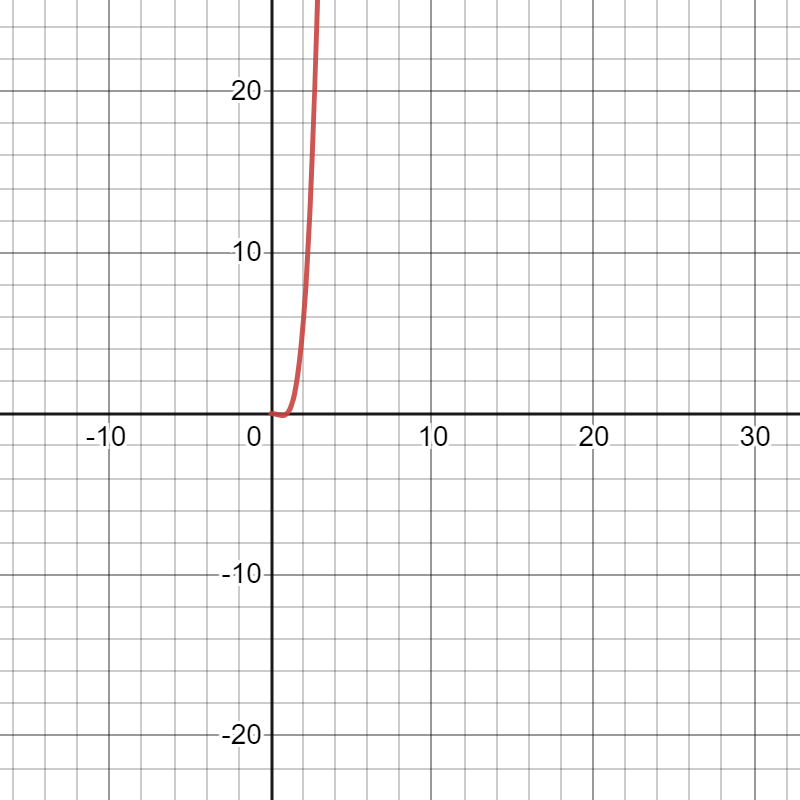
\includegraphics[scale=0.15]{2-3}}
\caption*{$ \alpha = -3 $}
\end{figure}\\
\begin{figure}[h!]
\center{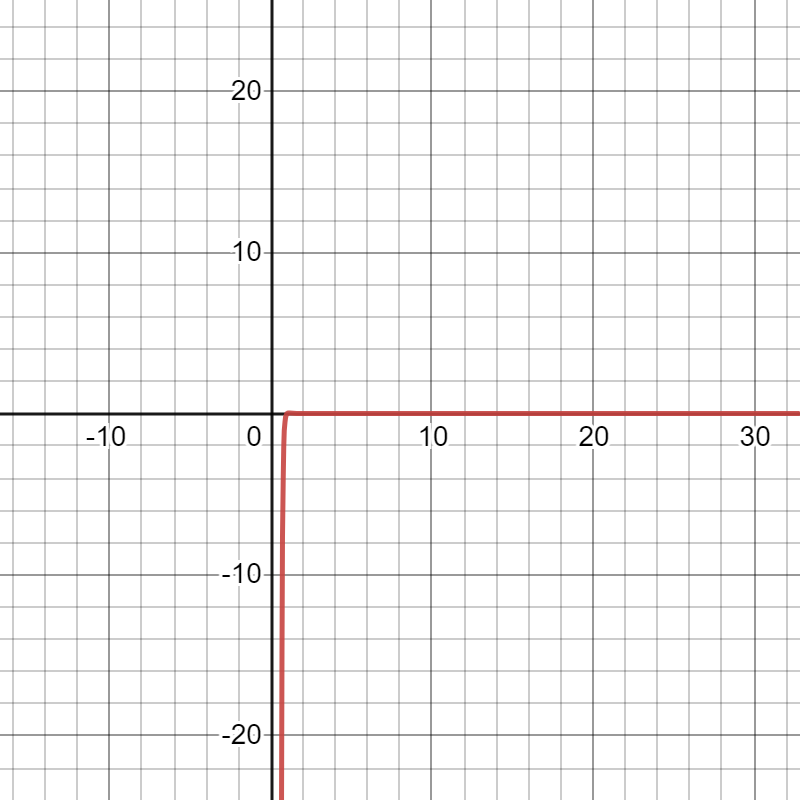
\includegraphics[scale=0.15]{210}}
\caption*{$ \alpha = 10 $}
\end{figure}\\
\begin{figure}[h!]
\center{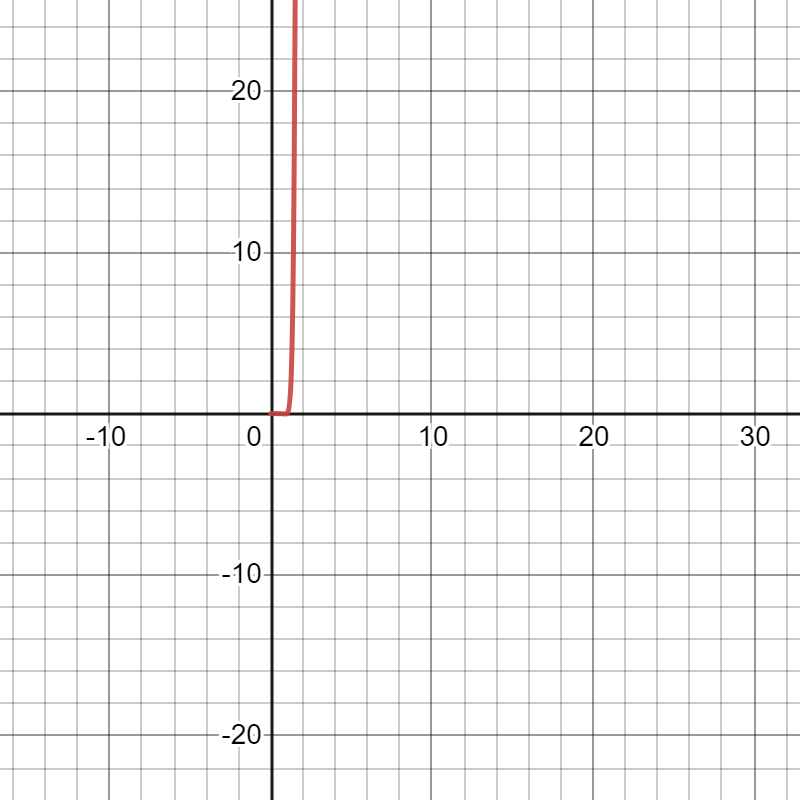
\includegraphics[scale=0.15]{2-10}}
\caption*{$ \alpha = -10 $}
\end{figure}\\
3. При $ \alpha = 0 $:\\
\large
$ \int\limits \frac{\ln{x}}{x^{\alpha}}dx = \int\limits \frac{\ln{x}}{x^0}dx = \int\limits \ln{x}dx = u\upsilon - \int\limits ud\upsilon = x\ln{x} - \int\limits x\frac{1}{x}dx = x\ln{x} - x + C = x(\ln{x} - 1) + C = f(x) = \lim_{x\to \infty} f(x) = \infty => $ расходится\\
\normalsize
При $ \alpha = 1 $:\\
\large
$ \int\limits \frac{\ln{x}}{x}dx = \int\limits udu = \frac{u^2}{2} + C = \frac{\ln^2{x}}{x} + C $\\
\normalsize
При $ \alpha \in Z $: берётся по частям\\\\\\\\
4. Признаки сравнения:\\
Первый признак сравнения:\\
Если на промежутке $ [a; +\infty) $ непрерывные $ f(x) $ и $ g(x) $ удовлетворяют условию:\\
$ 0 \le f(x) \le g(x) $, то из сходимости интеграла $ \int\limits^{+\infty}_{a} g(x)dx $ следует сходимость интеграла $ \int\limits^{+\infty}_{a} f(x)dx $, а из расходимости интеграла $ \int\limits^{+\infty}_{a} f(x)dx $ следует расходимость интеграла $ \int\limits^{+\infty}_{a} g(x)dx $\\
Второй признак сравнения:\\
Если существует предел $ \lim_{x\to \infty} \frac{f(x)}{g(x)} = k $:\\
$ (0 < k < \infty, f(x) > 0 $ и $ g(x) > 0) $, то интегралы $ \int\limits^{+\infty}_{a} f(x)dx $ и $ \int\limits^{+\infty}_{a} g(x)dx $ одновременно оба сходятся или оба расходятся
\Large
\section{Приложения определенного интеграла}
\normalsize
Найти давление воды на поверхность цилиндра диаметром 4м и высотой 6м, если его верхнее основание находится на уровне свободной поверхности воды.
\Large
\section{Приближенные вычисления определенного интеграла}
\normalsize
Вычислить значения интеграла $ I^2_0 = \int\limits^2_0 f(x)dx $ по формулам трапеций и парабол при $ h = 1 $, сравнить полученные результаты с точным значением. В качестве подынтегральных функций взять:

a) $ f(x) = 1 + x $

b) $ f(x) = 1 + x^3 $

\end{document}